\documentclass[10pt,a4paper]{article}
\usepackage{fontawesome}
\usepackage{hyperref}
\usepackage{graphicx}
\usepackage{academicons}
\usepackage{hyperref}
\usepackage{hanging}
\usepackage{geometry}
\usepackage[utf8]{inputenc}
\usepackage[T1]{fontenc}
\usepackage{doi}
\usepackage[style=apa, sorting=ynt]{biblatex}
\usepackage{enumitem}
\usepackage{amsmath}
\usepackage{MnSymbol}%
\usepackage{wasysym}%
\usepackage{makecell}
\usepackage{tabularx}
\usepackage{titlesec}

\geometry{left=1in,right=1in,top=1in,bottom=1in}
\setlength{\parindent}{0pt}
\setlist[itemize]{leftmargin=*,label=\small\raisebox{0.22ex}{$\blacksquare$}}

\titleformat{\section}
{\normalfont\Large\bfseries}{\thesection}{1em}{}[{\hrule}]

\addbibresource{publications.bib}

\title{\textsc{Curriculum Vitae}}
\date{}

\begin{document}
    \maketitle
    \begin{minipage}{.75\linewidth}
        \Large ir. \textbf{Arne Van Den Kerchove}\\
        \normalsize Doctoral Researcher at KU Leuven Neurophysiology Group

        \bigskip

        \begin{tabular}{@{}c l}
            \faAt        & \texttt{arne.vandenkerchove@kuleuven.be} \\
            \faPhone     & +32 473 32 78 71                         \\
            \faMapMarker & Research Group Neurophysiology,          \\
            & ON II Herestraat 49 - box 1021,          \\
            & BE-3000 Leuven                           \\
            \aiOrcid     & \url{orcid.org/0000-0002-9367-2986}      \\
            \faGlobe     & \url{arne.vandenkerchove.com}
        \end{tabular}
    \end{minipage}%
    \begin{minipage}{.25\linewidth}
        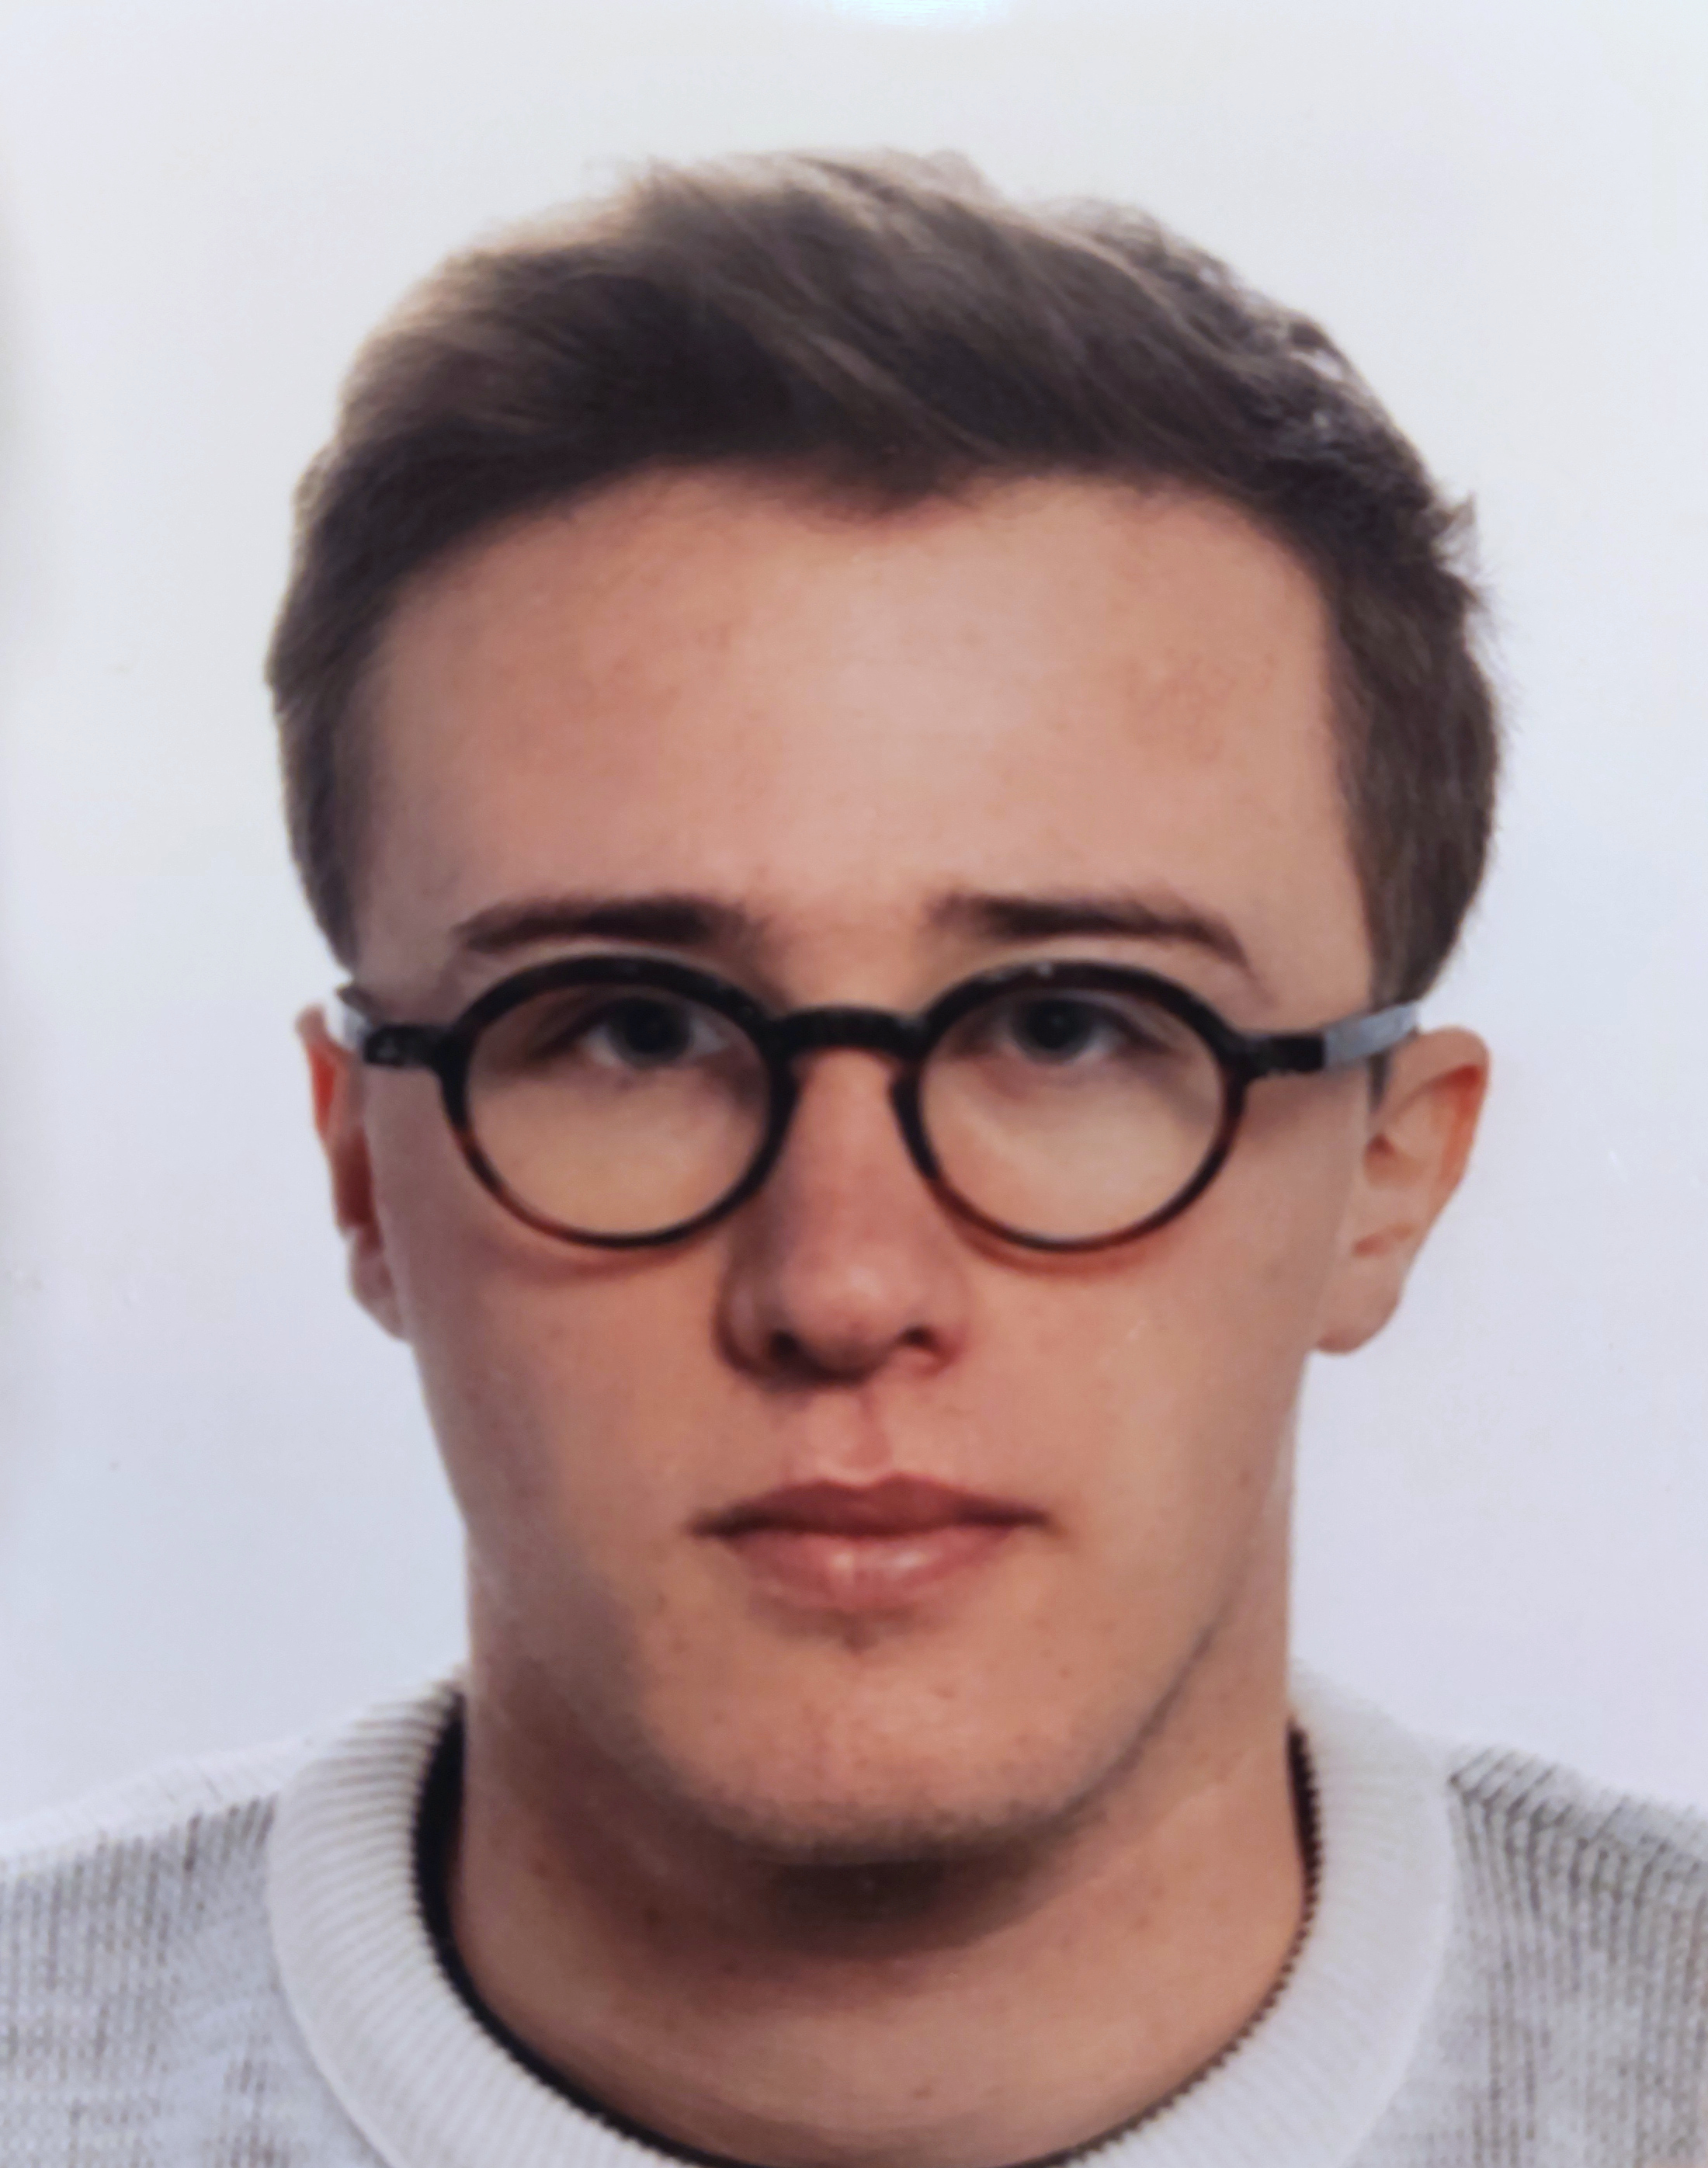
\includegraphics[width=\linewidth]{photo.jpg}
    \end{minipage}

    \paragraph{Research interests:} brain-computer interfaces, spatio-temporal beamforming, machine learning


    \bigskip
    \hrule
    \bigskip

    Ph.D. candidate at KU Leuven Laboratory for Neuro- and Psychophysiology and University of Lille CRIStAl
    Brain-computer Interface Team. My research focuses on ERP-based visual brain-computer interfaces for
    assisting patients with severe disabilities, combining machine learning, neurophysiology and
    user interface design.

    \section*{Education}
    \renewcommand{\arraystretch}{1.5}
    \begin{tabularx}{\linewidth}{@{}p{1.2in} X@{}}
        ongoing & Ph.D. in Biomedical Sciences, KU Leuven                             \\
        ongoing & Ph.D. in Control Science and Signal Processing, University of Lille \\
        2020    & M.Sc. in Engineering Science: Computer Science, KU Leuven           \\
        2017    & B.Sc. in Informatics, KU Leuven                                     \\
    \end{tabularx}


    \section*{Professional Experience}

    \begin{tabularx}{\linewidth}{@{}p{1.2in} X@{}}
        12/2020 - ongoing & Research Assistant, KU Leuven Neuro- and Psychophysiology Lab \\
        07/2019 - 12/2019 & \makecell[{{X}}t]{Python Developer, Mindspeller               \\
        Python Flask developer in a KU Leuven spin-off that provides neuromarketing services based on
        scientifically validated neuroscience and
        AI research.} \\
    \end{tabularx}


    \section*{Teaching Experience}

    \begin{tabularx}{\linewidth}{@{}p{1.2in} X@{}}
        02/2020 - 06/2020 & \makecell[{{X}}t]{Student Assistant Fundamentals of Computer Science, KU Leuven \\
        Teaching exercise sessions in Python programming and algorithmic reasoning to first year engineering students
        .} \\
        09/2015 - 01/2016 & \makecell[{{X}}t]{PAL tutor Principles of Computer Programming, KU Leuven       \\
        Organizing and teaching peer-assisted learning sessions in Python programming for first year Informatics
        students.} \\
    \end{tabularx}


    \section*{Funding}

    \begin{tabularx}{\linewidth}{@{}p{1.2in} X@{}}
        2020 & \makecell[{{X}}t]{KU Leuven and University of Lille Global Ph.D. Partnership Grant \\
        Proposal: \textit{EEG-based Visual Brain-Computer Interface for Gaze-free Communication}} \\

    \end{tabularx}

    \section*{Publications}


    \nocite{*}

    \printbibliography[heading=none]


\end{document}
